La cuve à ondes peut être utilisée comme dispositif pour étudier la propagation
des ondes. Selon les conditions de l'expérience, on peut assister aux phénomènes
de propagation et de diffraction ce qui permet d'identifier certaines
caractéristiques des ondes et du milieu de propagation.

À l'aide du vibreur de la cuve à ondes, on crée à $t_{0}=0$ en un point $S$ de
la surface libre de l'eau une onde progressive sinusoïdale de fréquence
$\freq=\qty{20}{\Hz}$.

\begin{enumerate}
    \item L'onde se propage à la surface de l'eau avec une célérité $v$ sans
          amortissement ni réflexion.
          \begin{enumerate}
              \item Définir une onde mécanique progressive sinusoïdale.
              \item L'onde étudiée est-elle longitudinale ou transversale~?
                    Justifier.
          \end{enumerate}
    \item \mbox{}
          \begin{minipage}[t][][t]{0.76\linewidth}
              La figure ci-contre schématise l'aspect de la surface de l'eau à
              un instant $t$ où les cercles représentent les crêtes.

              Recopier, sur votre copie, le numéro de la question et choisir la
              lettre correspondante à la proposition vraie.
          \end{minipage}
          \hfill
          \begin{minipage}[t][][t]{0.20\linewidth}
              \begin{figure}[H]
                  \centering
                  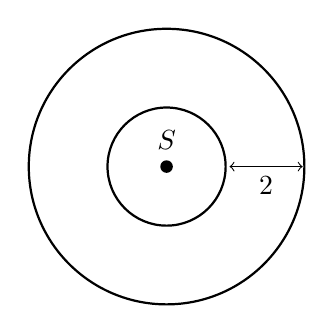
\begin{tikzpicture}[]
                      \node[circle,fill,inner sep=1.6pt,label=$S$] (S) {};
                      \node[circle,draw,thick,inner sep=0pt,
                            minimum size=1.5cm] (C1) {};
                      \node[circle,draw,thick,inner sep=0pt,
                            minimum size=3.5cm] (C2) {};
                      \draw[<->,shorten <=1pt,shorten >=1pt] (C1.east) -- 
                          node[below] {$\qty{2}{\cm}$} (C2.east);
                  \end{tikzpicture}
              \end{figure}
          \end{minipage}

          \vspace{-2cm}
          \begin{enumerate}
              \item La valeur de la longueur d'onde $\lambda$ est~:
          
                    \begin{enumerate*}[label=\fbox{\Alph{enumiii}},
                            itemjoin=\hspace{1cm}]
                        \item $\lambda=\qty{1}{\cm}$
                        \item $\lambda=\qty{1.5}{\cm}$
                        \item $\lambda=\qty{2}{\cm}$
                        \item $\lambda=\qty{2.5}{\cm}$
                    \end{enumerate*}
              \item La valeur de la vitesse de propagation de l'onde à la
                    surface de l'eau est~: \par
                    \begin{enumerate*}[label=\fbox{\Alph{enumiii}},itemjoin=\hfill]
                        \item $v=\qty{0.4}{\m\per\s}$
                        \item $v=\qty{0.3}{\m\per\s}$
                        \item $v=\qty{0.2}{\m\per\s}$
                        \item $v=\qty{0.15}{\m\per\s}$
                    \end{enumerate*}
          
              \item Les points situés à la distance $d=\qty{4}{\cm}$ de $S$
                    sont atteints par l'onde à l'instant $t_{1}$.
          
                    La valeur de $t_{1}$ est~: \par
                    \begin{enumerate*}[label=\fbox{\Alph{enumiii}},itemjoin=\hfill]
                        \item $t_{1}=\qty{0.2}{\s}$
                        \item $t_{1}=\qty{0.15}{\s}$
                        \item $t_{1}=\qty{0.1}{\s}$
                        \item $t_{1}=\qty{0.05}{\s}$
                    \end{enumerate*}
          \end{enumerate}


    \item On considère le point $M$ de la surface de l'eau situé au repos à la
          distance $d=\qty{4}{\cm}$ de la source $S$. Écrire l'élongation
          $y_{M}(t)$ du point $M$ en fonction de l'élongation de la source $S$.
  
    \item On règle la fréquence du vibreur sur la valeur
          $\freq^{\prime}=\qty{10}{\Hz}$, on obtient à la surface de l'eau une onde
          de longueur d'onde $\lambda^{\prime}=\qty{3}{\cm}$. Déduire, en
          justifiant la réponse, une propriété du milieu de propagation.
    \item On excite à nouveau la surface de l'eau avec une réglette mince, on
          obtient une onde rectiligne progressive périodique de fréquence
          $\freq=\qty{20}{\Hz}$ qui se propage à la vitesse
          $v=\qty{0.4}{\m\per\s}$.

          On place un obstacle muni d'une ouverture de largeur
          $a=\qty{0.5}{\cm}$ sur le trajet des ondes.
          \begin{enumerate}
              \item Justifier que l'onde subit la diffraction après la traversée
                    de l'ouverture.
              \item Donner les caractéristiques de l'onde après la traversée de
                    l'ouverture.
          \end{enumerate}
\end{enumerate}

